\documentclass[10pt,a4paper]{article}
\usepackage[margin=18mm,headheight=14pt,headsep=7mm,footskip=10mm]{geometry}
\usepackage[T1]{fontenc}
\usepackage{lmodern,amsmath,booktabs,array,xcolor,fancyhdr,hyperref,pgfplots,graphicx}
\pgfplotsset{compat=1.18}
\definecolor{Navy}{HTML}{17354B}\definecolor{Teal}{HTML}{166979}
\hypersetup{colorlinks=true,urlcolor=Teal,linkcolor=Teal,pdftitle={Estimated nickel tearing law},pdfauthor={MIT Rocket Team -- exploratory simulation}}
\pagestyle{fancy}\fancyhf{}
\fancyhead[L]{\small\color{Navy}MIT Rocket Team \enspace | \enspace Power board}
\fancyhead[R]{\small\color{Navy}Nickel tearing estimate}
\fancyfoot[L]{\footnotesize 6 October 2026 \enspace | \enspace Working draft / simulation in progress}
\fancyfoot[R]{\footnotesize\thepage}
\renewcommand{\headrulewidth}{0.3pt}
\setlength{\parindent}{0pt}\setlength{\parskip}{5pt}\setlength{\emergencystretch}{2em}
\renewcommand{\arraystretch}{1.15}
\newcommand{\ReportHeading}[1]{\par\vspace{6pt}{\large\bfseries\color{Teal}#1}\par\vspace{3pt}}
\newcommand{\PageTitle}[1]{{\LARGE\bfseries\color{Navy}#1\par}\vspace{7pt}}
\begin{document}
\PageTitle{Estimated nickel tearing law}
{\large\color{Teal}Material model and simulation study: working draft}\par
A usable first estimate is a \textbf{0.30 accumulated local equivalent plastic strain for damage initiation in simple tension}, followed by softening over \textbf{0.12 mm relative equivalent plastic displacement}. This is conditional on soft/annealed nickel. It is an engineering hypothesis for sensitivity analysis, not a fitted property of the user's strip and not a predicted battery breaking force.

\ReportHeading{Proposed inputs}
\begin{center}
\begin{tabular}{p{.45\linewidth}rrr}\toprule
Input & Lower value & Nominal & Upper value\\\midrule
Initiation strain at $\eta=1/3$, $\varepsilon_0$ & 0.10 & 0.30 & 0.60\\
Post-initiation displacement $u_f$ (mm) & 0.03 & 0.12 & 0.24\\
Triaxiality exponent $\beta$ & \multicolumn{3}{c}{1.5 assumed}\\
Strip thickness (mm) & \multicolumn{3}{c}{0.15 from model}\\\bottomrule
\end{tabular}
\end{center}
Vary initiation and evolution independently: the three-by-three combinations are sensitivity cases, not statistical confidence limits. The range does not bound spring-temper nickel or defects in an unknown weld.

Use the Granta annealed-sheet plasticity curve at 20$^\circ$C as the initial hardening model: 185 MPa yield and 102 exported points, ending at 530.429 MPa true stress and 0.199999 plastic strain. The source sheet is 0.787 mm thick; the modeled strip is 0.15 mm. Hardening past the exported endpoint is an additional assumption (page 3).

\ReportHeading{How the estimate was constructed}
The Granta source reports 40\% gauge-length elongation. Its logarithmic scale, $\ln(1.40)=0.336$, motivates a rounded initiation hypothesis of 0.30; it \emph{does not convert a tensile elongation measurement into a local fracture criterion}. The 0.10--0.60 interval deliberately explores that uncertainty.

Special Metals Table 13 reports 66\% and 78\% reduction in area at 21$^\circ$C for annealed Nickel 200 bars of 19 and 25.4 mm diameter [2]. Assuming locally incompressible uniaxial plastic flow gives an approximate final axial logarithmic strain
\[
\varepsilon_{\mathrm{local},f}\simeq-\ln(1-\mathrm{RA})
       =1.079\text{ to }1.514 .
\]
Using the lower bar value, an assumed localization-band width equal to the strip thickness, and the nominal onset produces
\[
u_f \simeq 0.15(1.079-0.30)=0.117\ \mathrm{mm}
          \;\longrightarrow\; \boxed{u_f=0.12\ \mathrm{mm}}.
\]
Transferring necked-bar ductility to thin sheet, ignoring neck triaxiality and using thickness as band width are substantial assumptions. This calculation supplies a scale, not a calibration. The solver's actual characteristic length must not be replaced by the strip thickness.

\clearpage
\PageTitle{Initiation and progressive damage}
Let $\eta=\sigma_m/\sigma_{\mathrm{eq}}$ be stress triaxiality, positive in hydrostatic tension. For nonnegative $\eta$, propose
\[
\varepsilon_i(\eta)=\varepsilon_0
       \exp[-1.5\max(\eta-1/3,0)],
\qquad
\omega=\int\frac{d\bar\varepsilon^p}{\varepsilon_i(\eta)}.
\]
Damage begins when $\omega=1$. The exponential is inspired by the Rice--Tracey void-growth dependence [3]; its normalization is estimated here. Holding the threshold constant below $\eta=1/3$ is a separate, uncalibrated low-triaxiality assumption. For the native implementation, an additional numerical extension sets the threshold to $10^6$ for $\eta\le-10^{-6}$, with a narrow linear transition to $\varepsilon_0$ at zero. This effectively suppresses compressive damage accumulation; it is an assumed tensile-tearing model, not a calibrated compression or shear failure law.

\begin{center}
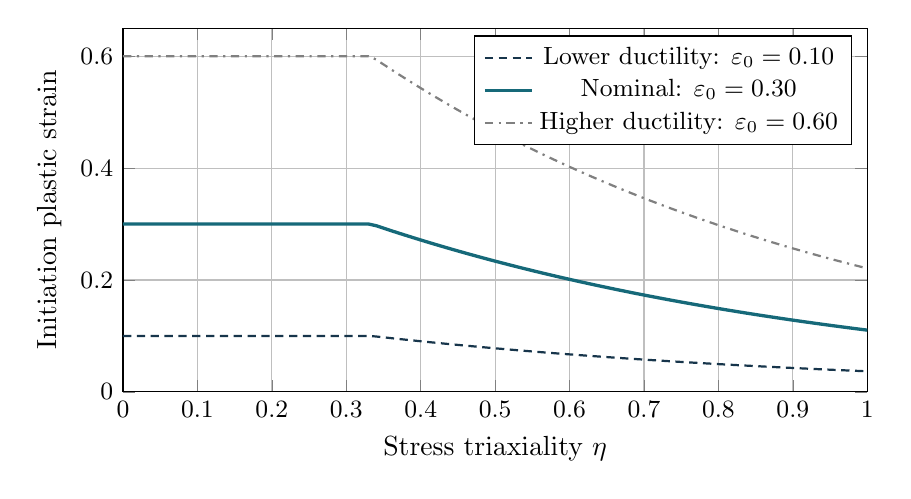
\begin{tikzpicture}
\begin{axis}[width=.91\linewidth,height=62mm,xmin=0,xmax=1,ymin=0,ymax=.65,
xlabel={Stress triaxiality $\eta$},ylabel={Initiation plastic strain},
grid=major,legend style={font=\small,at={(.98,.98)},anchor=north east},
tick label style={font=\small},samples=101]
\addplot[Navy,densely dashed,thick,domain=0:1] {.1*exp(-1.5*max(x-1/3,0))};
\addlegendentry{Lower ductility: $\varepsilon_0=0.10$}
\addplot[Teal,very thick,domain=0:1] {.3*exp(-1.5*max(x-1/3,0))};
\addlegendentry{Nominal: $\varepsilon_0=0.30$}
\addplot[gray,thick,dashdotted,domain=0:1] {.6*exp(-1.5*max(x-1/3,0))};
\addlegendentry{Higher ductility: $\varepsilon_0=0.60$}
\end{axis}
\end{tikzpicture}
\end{center}
{\small Curves are proposed assumptions drawn natively in \LaTeX; they are not test data or finite-element results.}

For constant $\eta$, the nominal threshold is 0.300 in simple tension, 0.182 at $\eta=2/3$, and 0.110 at $\eta=1$. A changing stress state requires the accumulated criterion; comparing one final strain maximum with one threshold is insufficient. The dependence omits Lode-angle effects, anisotropy and strain rate.

After initiation, use the provisional linear scalar law
\[
\bar u^p=\int_{\mathrm{onset}} L_{\mathrm{ch}}\,d\bar\varepsilon^p,\qquad
d=\min\!\left(\frac{\bar u^p}{u_f},1\right),\qquad
\boldsymbol\sigma=(1-d)\widetilde{\boldsymbol\sigma}.
\]
Here $L_{\mathrm{ch}}$ is the verified formulation's characteristic length and $\widetilde{\boldsymbol\sigma}$ is the effective elastoplastic stress. Full degradation of one material point does not establish a complete tear across a strip.

As a scale check, constant effective stress of 530 MPa with nominal linear softening gives $\tfrac12\sigma u_f\approx32$ N/mm of post-initiation work per unit area. This is an approximate consequence of the assumed law, not a measured fracture energy or the Granta toughness value.

\clearpage
\PageTitle{Reproduction and interpretation}
\ReportHeading{Hardening beyond the measured proxy}
The exported curve ends before nominal initiation in simple tension. Two explicit continuations are proposed for sensitivity:
\[
\sigma_{\mathrm{eff}}(p)=530.429\ \mathrm{MPa},
\quad\text{or}\quad
\sigma_{\mathrm{eff}}(p)=530.429
\left(\frac{p}{0.199999}\right)^{0.316193}\ \mathrm{MPa}
\quad(p>0.199999).
\]
The exponent comes from a log--log regression of the exported curve over $p\ge0.15$, with continuation anchored to its endpoint. At $p=0.30$ the power-law stress is approximately 603 MPa. Neither continuation is measured post-necking behavior; they are alternatives, not guaranteed bounds. The supplied table stops at $p=1.6$; native MISO holds the final stress constant beyond that point. Results exceeding 1.55 reported section-summary plastic strain are flagged because they approach the end of the tabulated hardening range. This summary does not bound every integration point. The corrected continuous-solution sequence has no live strain-limit stop.

\ReportHeading{Reproducible procedure}
Run \texttt{reproduce\_estimate.py} in the companion study folder. It reads the preserved Granta CSV, computes the reduction-of-area scale and tail exponent, and writes parameter JSON, initiation and assumed-hardening CSVs, and arithmetic validation. It neither modifies nor launches ANSYS.

The attachment input decks retain the two 750 N clamps, the edge-battery loading and nickel-only battery connection. They apply the candidate plasticity and damage models to the nickel, and increase prescribed battery displacement beyond the previous 0.5 mm endpoint. Track force, damage initiation, a connected tear path, and load drop separately. Compare all nine initiation/evolution pairs, both assumed hardening continuations and local mesh refinement. Include contact slip, clamp compliance and joint failure if they govern the result.

ANSYS 2026 R1 native ductile CDM is paired here with multilinear isotropic hardening, finite-deformation SHELL181 and \texttt{NLGEOM,ON}. The plasticity reference permits this combination using Cauchy stress and logarithmic strain. Three coupon checks reproduced damage initiation and progressive softening; all eventually stopped with excessive-thickness-change errors. The revised full-integration coupon reached damage 0.99323. The original attachment run was rejected after a load-history defect was found. A corrected continuous-solution proof passed with 23 converged states and four consecutive load steps. The strict full-attachment pull reached first damage near 43 N before force nonconvergence. Its converged subset passes the independent audits; sensitivity studies remain in progress. See the verification section for the converged-only results. The damage cap is 0.9999; no elements are deleted. Shell regularization uses in-plane integration, not thickness. The native proof uses logarithmic strain consistency as an independent check [5].

\ReportHeading{What the existing result establishes}
The first attachment implementation left the solution processor for postprocessing after each pull point. The native log then restarted subsequent pulls at load step 1 instead of preserving the preceding nonlinear state. Its force values are withdrawn as progressive-tearing predictions. The earlier bilinear comparison is also excluded pending a load-history audit. The rejected run was stopped through the native nonlinear abort mechanism at the user's request; inputs, diagnostics and restart evidence are preserved.

\ReportHeading{Sources and provenance}
{\small
[1] Granta Selector 2026 R1, Metals plus / JAHM Curve Data, \emph{Nickel 200, annealed sheet}; exported 5 October 2026. Record source: ASM International (2002), p.~631, Fig.~Ni.001. Local audit:
\path{outputs/granta_audit_20261005/granta_nickel_audit.txt}.\par
[2] Special Metals, \emph{Nickel 200}, Table 4 (elastic constants) and Table 13 (annealed-bar reduction in area). \href{https://www.specialmetals.com/documents/technical-bulletins/nickel-200.pdf}{Manufacturer bulletin}.\par
[3] Rice and Tracey (1969), \emph{On the ductile enlargement of voids in triaxial stress fields}, JMPS 17, 201--217. \href{https://doi.org/10.1016/0022-5096(69)90033-7}{Original theory}. The curve amplitude and low-triaxiality plateau in this addendum are analyst choices, not nickel constants from this paper.\par
[4] ANSYS 2026 R1, Material Reference, section 4.25.7, \href{https://ansyshelp.ansys.com/public/Views/Secured/corp/v261/en/ans_mat/mat_damageall.html}{Ductile Damage}.\par
[5] ANSYS 2026 R1, Material Reference, section 4.4.1.6, \href{https://ansyshelp.ansys.com/public/Views/Secured/corp/v261/en/ans_mat/amp8sq21dldm.html}{Small-strain plasticity in large-deformation analyses}.\par
[6] ANSYS 2026 R1, Command Reference, \href{https://ansyshelp.ansys.com/public/Views/Secured/corp/v261/en/ans_cmd/Hlp_C_CNVTOL.html}{CNVTOL}. The force tolerance multiplies a reference norm; it is not a direct percentage error on the reported battery force.\par
Companion inputs and arithmetic:
\texttt{outputs/tearing\_estimate\_20261005/sources/}.\par
}
\clearpage
\PageTitle{Material-law verification}
Three native tensile-coupon runs used the same estimated material. The coupon is a 1 mm square, 0.15 mm thick; its force is \textbf{not the battery attachment force}. All curves below exclude ANSYS's unconverged debugging result set (substep 999999).

\begin{center}
\begin{tikzpicture}
\begin{axis}[width=.93\linewidth,height=63mm,xlabel={Coupon extension (mm)},ylabel={Coupon tensile force (N)},
grid=major,xmin=0,ymin=0,legend style={font=\footnotesize,at={(.98,.98)},anchor=north east},tick label style={font=\small}]
\addplot[Navy,thick] table[x=ux_mm,y=fx_N,col sep=comma]{tearing_data/coupon_nominal_v4.csv};
\addlegendentry{Full integration: initial settings}
\addplot[Teal,dashed,thick] table[x=ux_mm,y=fx_N,col sep=comma]{tearing_data/coupon_unsym.csv};
\addlegendentry{Full integration: revised settings}
\end{axis}
\end{tikzpicture}

\begin{tikzpicture}
\begin{axis}[width=.93\linewidth,height=63mm,xlabel={Accumulated plastic strain},ylabel={Damage $d$},
grid=major,xmin=.25,xmax=.54,ymin=0,ymax=1,legend style={font=\footnotesize,at={(.02,.98)},anchor=north west},tick label style={font=\small}]
\addplot[Navy,thick] table[x=eppl,y=damage,col sep=comma]{tearing_data/coupon_nominal_v4.csv};
\addlegendentry{Full integration: initial}
\addplot[Teal,dashed,thick] table[x=eppl,y=damage,col sep=comma]{tearing_data/coupon_unsym.csv};
\addlegendentry{Full integration: revised}
\addplot[gray,dashdotted,thick] table[x=eppl,y=damage,col sep=comma]{tearing_data/coupon_uniform.csv};
\addlegendentry{One in-plane point, uniform edge}
\end{axis}
\end{tikzpicture}
\end{center}

The revised full-integration proof reached 456 converged states: fitted damage onset 0.30203, final damage 0.99323, and maximum logarithmic-strain consistency residual $1.53\times10^{-6}$. Peak coupon force changed from 66.870 to 66.891 N (0.031\%) when the solver and substep controls were tightened.

The one-point uniform-edge diagnostic reached damage 0.98619 and fitted onset 0.30055. Its steeper damage curve reflects the different in-plane characteristic length; it does not replace the fully integrated attachment mesh. All three runs eventually stopped with excessive shell-thickness-change errors. These checks support initiation and nearly complete softening, but do not establish robust continuation through zero stiffness or geometric separation.

\clearpage
\PageTitle{Verification of the preload history}
A one-core attachment proof carries preload, locking and two pull increments through one uninterrupted solution session. Its native log and independently extracted result sets agree on the sequence: load steps 1, 2, 3 and 4, with 23 converged substeps and no native errors.

\begin{center}
\begin{tabular}{p{.65\linewidth}r}\toprule
Verification quantity & Result\\\midrule
Each clamp reaction immediately after locking & 750.000 N\\
Sideways displacement at the final proof state & 0.500 mm\\
Lateral battery reaction at that state & 11.333 N\\
Each clamp reaction after the pull & 768.950 N\\
Maximum reported equivalent plastic strain & 0.01124\\
Maximum reported damage & 0\\
Worst relative X force imbalance & 0.0282\%\\
Worst absolute Z force imbalance & 0.0126 N\\\bottomrule
\end{tabular}
\end{center}
The clamp reactions increase after locking because platen separation is fixed while the strips deform. The 750 N value is the initial preload, not a constant force maintained throughout pulling. The 11.333 N value is an elastic--plastic response check, not a tearing load or an observed force maximum beyond the proof interval.

\begin{center}
\begin{tikzpicture}
\begin{axis}[width=.93\linewidth,height=70mm,xlabel={Battery sideways displacement (mm)},ylabel={Battery lateral reaction (N)},
grid=major,xmin=0,xmax=.5,ymin=0,tick label style={font=\small}]
\addplot[Teal,very thick,mark=*,mark size=1.1pt] table[x=ux_mm,y=fx_N,col sep=comma]{tearing_data/continuous_proof.csv};
\end{axis}
\end{tikzpicture}
\end{center}
Native convergence warnings were retained and reviewed. They concern constraints at the common rigid battery pilot, the inherited nickel section reference on a contact element, and sparse-solver pivoting. No negative-pivot or constraint failure occurred. Finite result fields, the locked-preload reactions and independent force balance pass the stated checks.

The rejected earlier implementation is not restarted or reused as a solution checkpoint. Corrected cases begin from fresh sealed model inputs. A guard checks the cumulative load-step number after every solve, and the result audit rejects resets in time, load-step number or cumulative iterations.


% BEGIN VALIDATED NOMINAL RESULTS
\clearpage
\PageTitle{First attachment damage: validated partial run}
The strict nominal run preserves all preload and deformation history, but stops before the requested 8 mm endpoint. The retained 110 converged states span 16 consecutive load steps. \textbf{Damage is detected near 43 N; a breaking load has not been established.} The final reaction is still increasing, so its maximum is only the largest force observed before nonconvergence.

\begin{center}
\begin{tabular}{p{.62\linewidth}r}\toprule
Quantity & Strict nominal result\\\midrule
First detectable damage displacement bracket & 3.250--3.275 mm\\
Reaction across that bracket & 42.870--43.372 N\\
Last converged displacement / reaction & 3.3474 mm / 44.857 N\\
Maximum reported damage at that state & 0.00887\\
Maximum reported equivalent plastic strain & 0.19941\\
Final normal reaction at each locked clamp & 871.43 N\\
Worst X force imbalance / relative imbalance & 0.00233 N / 0.0282\%\\
Worst Y / Z force imbalance & 0.0000061 N / 0.0127 N\\\bottomrule
\end{tabular}
\end{center}
Detectable onset here means maximum top/mid/bottom element-summary damage exceeds $10^{-4}$. This brackets a reporting threshold; it is not the exact first damaged integration point. The first damage occurs in the flat strip beside the sharp bend, outside the washer footprint. No severed strip or postpeak force drop is demonstrated.

An early stable copy of the ongoing tolerance-sensitivity run contains 128 validated converged states, reaching 3.3604 mm and 45.138 N. Over the shared 0.025--3.3474 mm interval, its force differs by at most 0.0102\%, the clamp reactions by 0.0065\%, and summary damage by $3.46\times10^{-5}$. Both runs detect damage in the same displacement interval. This early subset satisfies the independent force-balance limits. It supports agreement over the shared interval, not an uncomputed peak or acceptance of later states.

\begin{center}
\begin{tikzpicture}
\begin{axis}[width=.93\linewidth,height=64mm,xlabel={Battery sideways displacement (mm)},ylabel={Battery lateral reaction (N)},
grid=major,xmin=0,xmax=3.5,ymin=0,tick label style={font=\small}]
\addplot[Teal,very thick] table[x=ux_mm,y=fx_N,col sep=comma]{tearing_data/cont_nominal.csv};
\addplot[Navy,only marks,mark=*,mark size=2pt] coordinates {(3.275,43.37207)};
\node[anchor=south east,font=\small] at (axis cs:3.22,44) {Damage detected};
\end{axis}
\end{tikzpicture}
\begin{tikzpicture}
\begin{axis}[width=.93\linewidth,height=49mm,xlabel={Battery sideways displacement (mm)},ylabel={Maximum summary damage},
grid=major,xmin=3.2,xmax=3.4,ymin=0,ymax=.01,tick label style={font=\small},scaled y ticks=false]
\addplot[Navy,thick,mark=*,mark size=1pt] table[x=ux_mm,y expr={max(\thisrow{dtop},max(\thisrow{dmid},\thisrow{dbot}))},col sep=comma]{tearing_data/cont_nominal.csv};
\end{axis}
\end{tikzpicture}
\end{center}

\clearpage
\PageTitle{Damage location and numerical limit}
\begin{center}
\includegraphics[width=.85\linewidth]{tearing_figures/cont_nominal_step101_assembly_detail.png}

\includegraphics[width=.64\linewidth]{tearing_figures/cont_nominal_step101_washer_detail.png}
\end{center}
{\small Both external figures show the last converged strict-nominal state. The detailed colour range is 0--0.01, not 0--1. Assembly deformation is at true scale; the lower panel uses undeformed material coordinates. The highlighted region lies near the bend, beyond the washer outer edge.}

At the last state, maximum contact pressure is 91.72 MPa and reported accumulated tangential motion is 0.00500 mm. All 3072 contact elements are accounted for: 1536 have a highest integration-point status of sticking, and 1536 are open. These element statuses do not exclude slip at individual integration points or represent contact area fractions.

The solve terminates at an attempted 3.3475 mm displacement: force residual 0.02709 N exceeds the 0.01751 N criterion after 60 iterations and cutback to a 0.000125 mm increment. Displacement and moment criteria pass. The unconverged debugging set is excluded. This numerical termination is not evidence of a tear. The tolerance-sensitivity run also terminated with force nonconvergence, at an attempted 3.53928125 mm. Its early subset agrees with the strict run, but later states fail the independent equilibrium check described next. The finer-mesh comparison is running; mesh, material and direction findings remain outstanding.
% END VALIDATED NOMINAL RESULTS

\clearpage
\PageTitle{Independent equilibrium check}
The tolerance trial changes only the pull force-convergence tolerance from $10^{-5}$ to $5\times10^{-5}$; preload retains $10^{-5}$. This allows further native convergence, but it does not ensure that every later result satisfies the separate study checks. The acceptance limits were kept unchanged: X imbalance divided by $\max(|F_X|,1\,\mathrm{N})$ below 0.001, Y imbalance below 0.01 N, and Z imbalance below 0.10 N.

The trial ended on 7 October at 02:02 EDT with force nonconvergence. Separate native extraction has zero errors and contains 794 converged states, including 785 pull states, through 3.5391562 mm. The 750 N locking reactions and continuous load history pass their checks. However, \textbf{339 pull states exceed the vertical force-balance limit}. The later response is rejected; its diagnostic endpoint of 49.069 N is neither a validated maximum nor a breaking load.

\begin{center}
\begin{tabular}{p{.64\linewidth}r}\toprule
Diagnostic quantity & Recorded value\\\midrule
First displacement exceeding the Z limit & 3.40133 mm\\
Largest absolute Z reaction sum & 0.80115 N\\
Displacement at that largest imbalance & 3.41735 mm\\
Predetermined Z acceptance limit & 0.10000 N\\
Largest absolute Y reaction sum & 0.0011315 N\\\bottomrule
\end{tabular}
\end{center}

\begin{center}
\begin{tikzpicture}
\begin{axis}[width=.94\linewidth,height=82mm,xlabel={Battery sideways displacement (mm)},ylabel={Sum of vertical support reactions (N)},
grid=major,xmin=3.2,xmax=3.55,ymin=-.9,ymax=.9,tick label style={font=\small},
legend style={font=\footnotesize,at={(.02,.98)},anchor=north west}]
\addplot[Navy,thick] table[x=ux_mm,y=rz_N,col sep=comma]{tearing_data/cont_nominal_balance.csv};
\addlegendentry{Strict nominal: accepted subset}
\addplot[Teal,thin,mark=*,mark size=.65pt] table[x=ux_mm,y=rz_N,col sep=comma]{tearing_data/cont_force5em5_balance.csv};
\addlegendentry{Tolerance trial: rejected later response}
\addplot[red,dashed,domain=3.2:3.55] {.1};
\addlegendentry{Unchanged $\pm0.10$ N limits}
\addplot[red,dashed,domain=3.2:3.55,forget plot] {-.1};
\end{axis}
\end{tikzpicture}
\end{center}
{\small Native \LaTeX\ graph from external CSV exports; no violating points are removed. The entire extracted pull history is retained; the unconverged debug set is excluded.}

An independent native \texttt{PRRSOL,F} listing from the earlier read-only snapshot, at load step 16, substep 138, confirms a 0.36828 N total using all reaction nodes. Separate listings of the four clamp pilots and the battery pilot give the same total. This rules out an omitted support reaction in the export as the explanation for this state. No acceptance threshold has been relaxed. Further diagnostic or revised numerical work is required before claiming a validated continuation; native convergence alone is insufficient [6].

\clearpage
\PageTitle{Attachment model and load sequence}
\begin{center}\includegraphics[width=.98\linewidth]{tearing_figures/model_overview.png}\end{center}
\ReportHeading{Geometry and constraints}
The elastic constants are $E=205$ GPa and $\nu=0.29$, matching the manufacturer's nominal annealed-nickel values at 26$^\circ$C [2]; they are held constant for this 20$^\circ$C study. 

The isolated model reconstructs the selected edge battery (CAD body 20157) and two nickel strips (bodies 20091 and 20348). Each strip is 0.15 mm thick and about 15 mm wide, with a sharp 90-degree bend. The hole radius is 2.704 mm; the washer outer radius is 5.5626 mm. These are model dimensions, not new measurements. Existing CAD gaps are assumed seated.

The battery is represented by rigid links to its nickel attachment regions. No battery-to-PCB connection or contact is introduced. The backing and washer surfaces are rigid; PCB bending, bolt compliance, the actual spot-weld pattern and local weld fracture are excluded. Coulomb friction is 0.20, an analyst assumption. Broad rigid battery attachments and a sharp modeled bend can influence the location and force of damage initiation.

SHELL181 uses full in-plane integration, seven through-thickness integration points and stored top/middle/bottom summaries. CONTA174 with TARGE170 models the washer interfaces (augmented Lagrange, friction 0.20, normal stiffness factor 0.1, penetration tolerance factor 0.01 and pinball factor 0.2). The sealed native commands are authoritative; these contact settings are numerical assumptions. MPC184 uses the Lagrange-multiplier rigid-link formulation.

\begin{enumerate}
\item Hold the battery and ramp each of the two lower platens to 750 N normal force. This local model uses the two clamps of one edge battery, not all six full-board bolts.
\item Record the lower-platen axial displacements. Replace the two forces with those locked displacements in a separate equilibrium step. Subsequent clamp reactions may change as the strips deform.
\item Release battery translation in Y and Z and all three rotations. Prescribe only lateral X translation at its rigid pilot, near battery mid-height, increasing in 0.25 mm output increments. Load-step time is a numerical ramp parameter, not a measured loading speed.
\item Use internal automatic substeps, large deformation and the unsymmetric sparse Newton solver. Retain every converged substep and subsequently extract force, free motion, clamp reactions, plastic strain and damage. No physical damping or viscous material regularization is included.
\end{enumerate}

\clearpage
\PageTitle{Reproducing the native calculation}
\ReportHeading{Saved input is the authoritative definition}
The companion package separates source generators, sealed per-case inputs, solver evidence and exported results. Every case has \texttt{model.inp}, \texttt{preflight.dat}, \texttt{run.dat}, \texttt{config.json} and \texttt{input\_sha256.json}. Attachment cases also contain \texttt{mesh.json}. The complete material curve is embedded in each APDL deck; reproducing a sealed case does not require another Granta export.

Corrected cases use the \texttt{continuous\_solu\_v2} protocol. Preload is load step 1, locking is step 2 and the pull sequence occupies consecutive later steps. All solves occur in one uninterrupted \texttt{/SOLU} session. Postprocessing is separate and never changes the active nonlinear solution.

\ReportHeading{Run in ANSYS 2026 R1}
\begin{enumerate}
\item Create a fresh local Windows directory for the desired case. Copy its sealed inputs there. Do not overwrite a completed or failed runtime. Confirm file hashes against \texttt{input\_sha256.json}.
\item Invoke the native executable in that working directory with the following preflight arguments. This deck contains no \texttt{SOLVE}:
\begin{quote}\small\ttfamily
ANSYS261.exe -b nolist -s noread -smp -np 1 -p preppost\par
-j check -i preflight.dat -o preflight.out
\end{quote}
\item Require zero native preflight errors and the expected inventory: 4 nodes/1 element for the shell coupon, 4277/7700 for the coarse attachment, or 16229/30676 for the refined attachment. Shell counts alone are 2304 and 9216; remaining elements implement contacts and rigid links.
\item Once the structural license is free, run the coupon with one SMP core, or the attachment with four SMP cores:
\begin{quote}\small\ttfamily
ANSYS261.exe -b nolist -s noread -smp -np 4 -p ansys\par
-j tear -i run.dat -o run.out
\end{quote}
\item Preserve the entire runtime, including result and restart files. Read the error count and convergence history; a closing \emph{RUN COMPLETED} banner alone is insufficient. Do not relaunch a failed solve without diagnosis.
\item After the solver exits, run the sealed \texttt{post.dat} in a separate one-core PrepPost session with job name \texttt{post}. It reads the original result file and excludes unconverged debug substep 999999. Export and validate \texttt{history.csv}, \texttt{balance.csv}, \texttt{damage\_N.csv} and \texttt{nodes\_N.csv}. The supplied analysis checks consecutive native load steps, monotone result times and cumulative iterations, retained 750 N locking reactions, displacement history, finite fields, damage bounds and force balance. Rejected runs retain their error logs and are labeled separately from accepted states.
\end{enumerate}
The tested executable was \texttt{v261/ansys/bin/winx64/ANSYS261.exe}, release 2026 R1.02, build 26.1 UP20260202, Windows x64 in Parallels. Units are N, mm and MPa. Guest runtimes are named \texttt{C:\textbackslash Temp\textbackslash PBTear26\_<case>}.

\ReportHeading{Figures and report}
Figures use native exported displacements and damage summaries, with English labels. The grey battery outline follows a rigid fit to its solved attachment motion. Deformation is shown at true scale unless marked. Graphs use native \texttt{pgfplots} in \LaTeX\ and read external CSV data. Compile \texttt{nickel\_tearing\_estimate.tex} from its own directory with the accompanying \texttt{tearing\_figures} and \texttt{tearing\_data} folders; compile twice to resolve references.

\end{document}
